\chapter{Background and Research Outline}
As discussed in the previous chapter, humanity's survey efforts have so far yielded little result in identifying small NEA's. In this chapter, first some background on the problem of identifying NEA's is given in \autoref{sec:introduction_NEA}, as well as examples of past, current, upcoming, and proposed survey missions in \autoref{sec:introductionidentification} and \autoref{sec:introductionproposals}. From here, it will become clear what the problem is that we are attempting to solve, and how a multi-spacecraft system might accomplish this. These topics are discussed in \autoref{sec:problemstatement} and \autoref{sec:researchmultispacecraft}, respectively. From this, in \autoref{sec:researchquestions} a set of research questions will be derived to be studied in this report. Lastly, in \autoref{sec:reportstructure}, a short overview of the structure of the report will be provided.

\section{Near-Earth Asteroids}
\label{sec:introduction_NEA}
Asteroids are perhaps the most diverse object in the Solar system: ranging in size from tiny chips to dwarf planets such as Vesta and Ceres; from rocky compositions, to fully metallic monoliths, and composites in various elements and mineral shapes; from close to the Sun on short orbits, to distant eccentric long period trajectories. All of this greatly increases the complexity of surveying for near-Earth asteroid. Before continuing, the definition of a near-Earth asteroid will be given as follows: \textit{a near-Earth asteroid is any asteroid with a perihelion $q \leq 1.3 \mathrm{AU}$ and semi-major axis $a \leq 4.2 \mathrm{AU}$}. \\

Current knowledge of the asteroid population is based on past and current NEA surveys. The most important parameter to consider is the size-frequency distribution of the objects. After all, larger objects exhibit a larger impact energy and hence threat, but small objects are more common and harder to detect. A good representation for this size-frequency distribution is a power law as follows:
\begin{equation}
 \frac{dN}{dD_p} \propto D_p^{-k}
 \label{eq:sizefreqlaw}
\end{equation}
With exponent $k$ in the range of 2.95 - 3.5 (\cite{AsteroidSizeFrequency}). Commonly, the size of the asteroid can not be directly ascertained; the target is too small to accurately determine the size through optical observation. However, estimates can be made based on the absolute magnitude $H$ of the object by relation with an assumed albedo $p_v$ - Commonly, $p_v = 0.14$ is used as an approximation - using the relationship first derived by \cite{AsteroidSizeAlbedo}:
\begin{equation}
 D = \frac{1329 \mathrm{km}}{\sqrt{p_v}}\cdot 10^{-H/5}
 \label{eq:asteroidsize}
\end{equation}
As a result of the success of the spaceguard survey efforts, past efforts have more than likely identified all NEA's with $H \leq 15$, corresponsing to the \textit{flying mountains} several kilometers in diameter. Also, at smaller limiting diameters, a lot of NEA's have been - and continue to be - found. The surveys through which this is achieved will be discussed in further detail in \autoref{sec:introductionidentification}. Through a process of modelling the asteroid population, and simulating the performance of past surveys on it, followed by fitting the results, \cite{GranvikPopulation} have produced a parametric model of the NEA population. The distribution of orbital elements in this model can be seen in \autoref{fig:population_histogram}. \\

\begin{figure}[htbp]
 \centering
 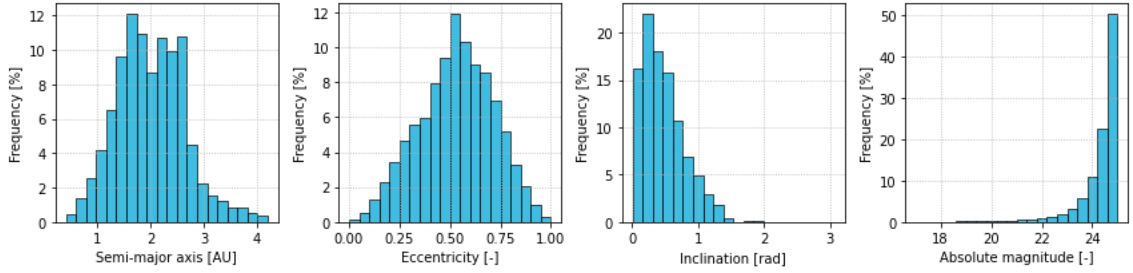
\includegraphics[width=1.0\textwidth]{img/population_histogram.png}
 \caption{Frequency of orbital elements for modelled NEA population according to \cite{GranvikPopulation}}.
 \label{fig:population_histogram}
\end{figure}

Several things are of note: First and foremost, the population is very diverse; there is no particular concentration of NEA's anywhere that allows for simple exploitation in survey design. Secondly, the bulk of NEA's has a semi-major axis of $1.0 \mathrm{AU} < a < 3.0 \mathrm{AU}$. The dips at $a = 2.0 \mathrm{AU}$ and $a = 2.5 \mathrm{AU}$ correspond to the 4:1 and 3:1 orbital resonance with Jupiter, respectively. The inclination of asteroids is concetrated among the ecliptic, but very low inclinations are rare due to gravitational interactions with the planets. Lastly, the effect of \autoref{eq:sizefreqlaw} can be seen: 50\% of the asteroids in the population generated by \cite{GranvikPopulation} has an absolute magnitude $24.6 \leq H < 25$, corresponding to a diameter of $D \leq 40 \mathrm{m}$. \\

Among these small NEA's was the asteroid which entered Earth's atmosphere over Chelyabinsk in 2013. It is currently estimated that this asteroid had a diameter of 17 to 20 meters (\cite{ChelyabinskNASA}). Assuming an albedo of $p_v = 0.14$, this results in an absolute magnitude of $H \approx 26.5$. As previously discussed, completeness at these limiting diameters is very low. \autoref{fig:completeness_size} shows the completeness as a function of size according to \cite{HarrisPopulation}. They estimate that, at their time of writing, less than 0.005\% of all asteroids of this size have been identified. Through new and continued survey efforts, \cite{2017NEOSDT} project that the completeness at this size will increase to approximately 1.5\% by 2023. \\

\begin{figure}[htbp]
 \centering
 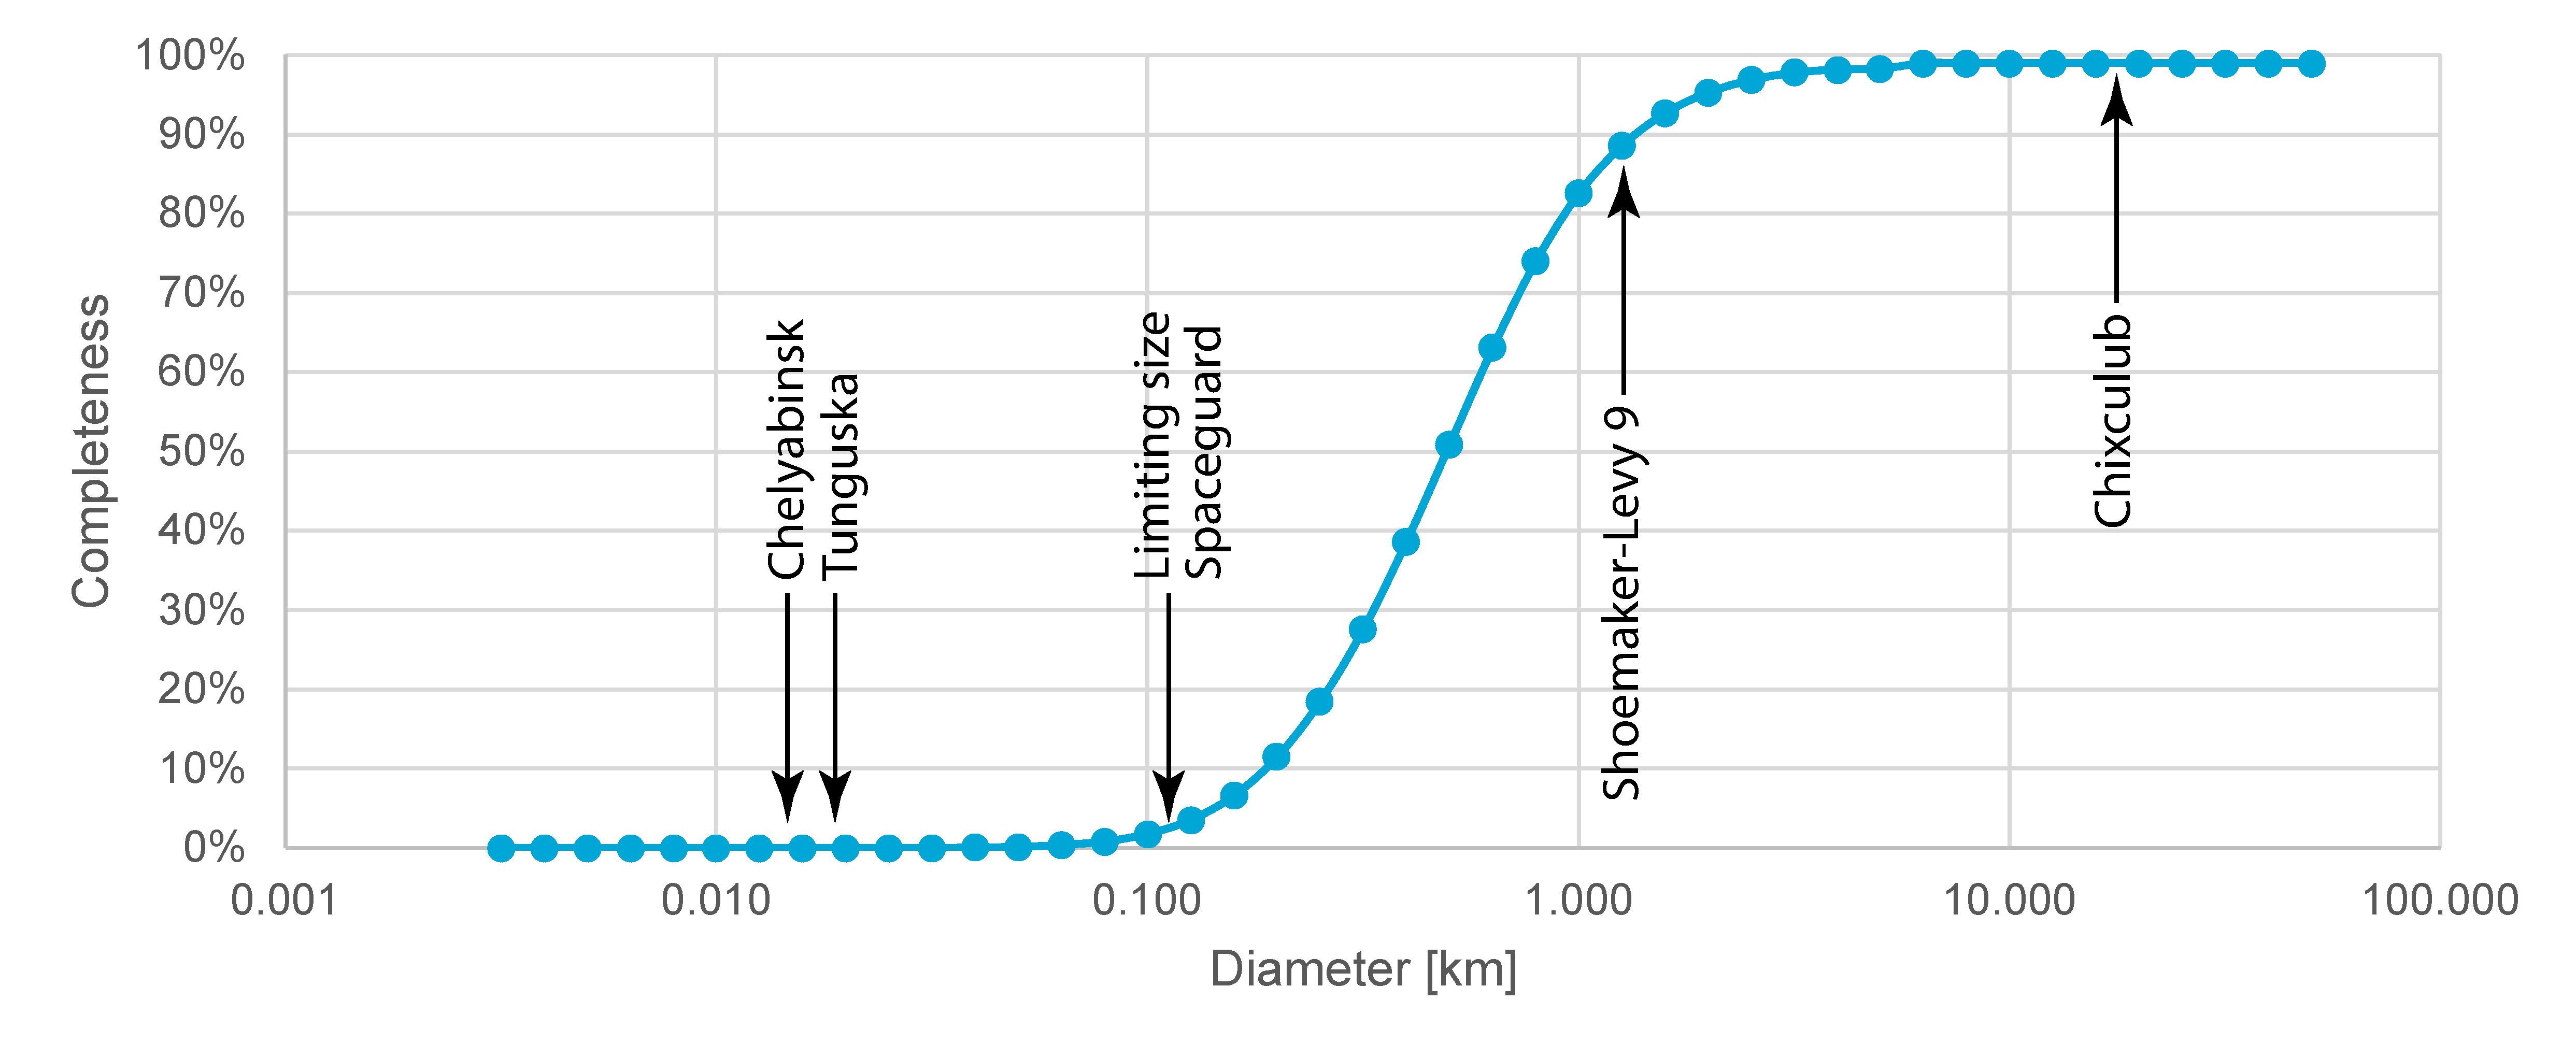
\includegraphics[width=0.8\textwidth]{img/completeness_size.pdf}
 \caption{Expected survey completeness as a function of near-Earth asteroid diameter. \cite{HarrisPopulation}}
 \label{fig:completeness_size}
\end{figure}

The problem can be seen in more detail in \autoref{fig:population_estimates}. Here, \cite{HarrisPopulation} show the expected and identified population of NEA's as a function of their size. The effect of the continued spaceguard efforts can be seen clearly here: the asteroid population with $D > 1 \mathrm{km}$ is completely known, and the population of asteroids $D > 140 \mathrm{m}$ is nearing the targeted 90\% completion. However, as the search efforts have been designed specifically to identify targets at this limiting size, the population with $D < 100 \mathrm{m}$ is still by far and large undiscovered.

\begin{figure}[htbp]
 \centering
 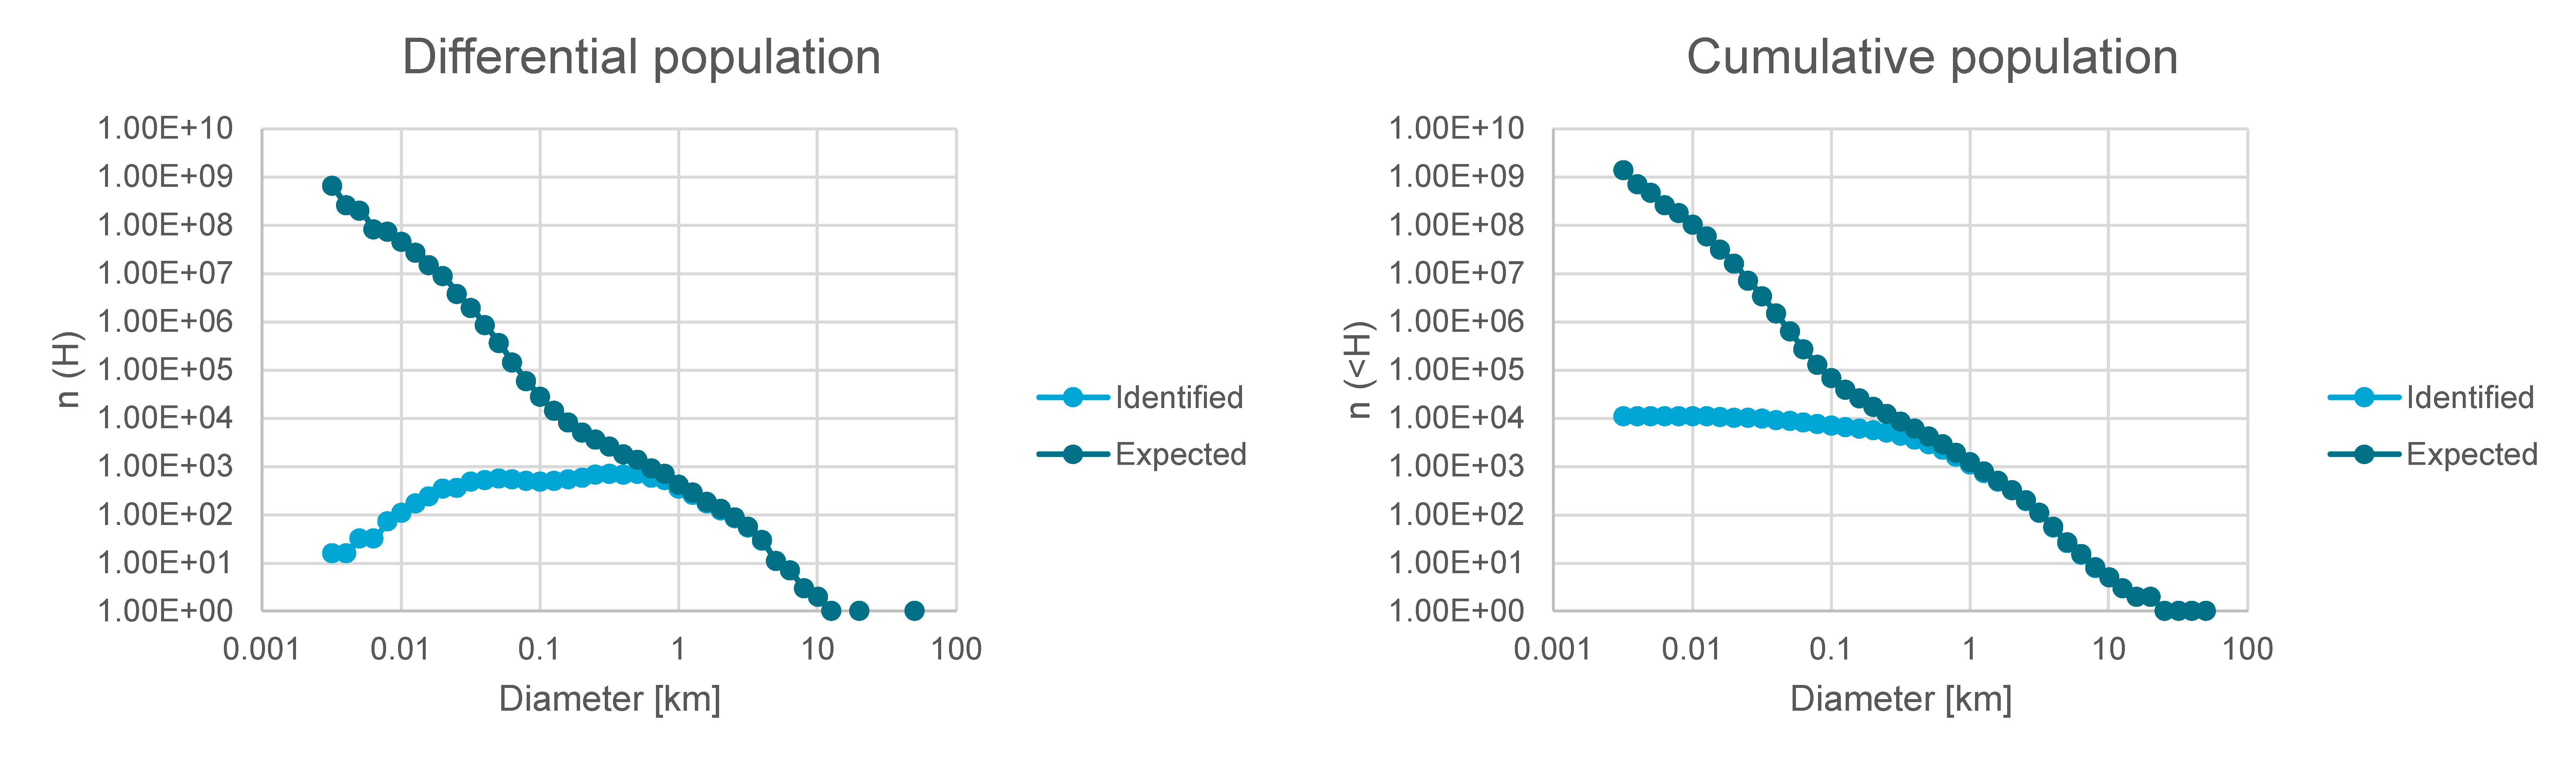
\includegraphics[width=1.0\textwidth]{img/population_estimates.pdf}
 \caption{State of asteroid identification progress as of August 2014, compared to the expected number of asteroids per diameter. Note that the y-axis is logarithmic. \cite{HarrisPopulation}}
 \label{fig:population_estimates}
\end{figure}


\section{Past and Current Identification Efforts}
\label{sec:introductionidentification}

Before continuing to the topic of the presented research, first some discourse shall be given to the missions that have resulted in the current knowledge of the NEA population. For brevity, not all missions will be listed, just a representative sample judged by the author to give a good overview of the state of the art. The missions are separated into two categories: space-based, and Earth-based. The latter comprises telescopes on Earth, with the advantage of having access to Earth infrastructure, supporting larger telescope apertures and providing practically unlimited electrical power, communication bandwidth, storage and computational resources. However, Earth-based systems are hindered by atmospheric distortion, extinction of light as it passes through the air, weather, limited search area depending on geographic position, and day-night cycles. Space-based systems contrast this: they are limited mostly by the maximum aperture of the telescopes they can support, the on-board processing capabilities and the computational power. Atmospheric and weather effects are mostly non-existant in space, however interference from the Sun, Earth and Moon should not be underestimated. To date, all NEA surveys from space have been carried out from orbits around Earth. Some proposals for deep space missions will be discussed in \autoref{sec:introductionproposals}.\\

In \autoref{fig:identification_per_survey}, the contribution of several surveys to the total catalogue of NEA's is shown. The two largest contributors, the Catalina Sky Survey and the Pan-STARRS observatories, were both constructed to accomplish the goal of bringing the NEA survey completeness for asteroids $D > 140 \mathrm{m}$ to over 90\% of the population. The effect of these purpose-built observatories can be easily seen in their volume of discoveries. Through improvement to the facilities and processing pipelines - e.g. through better computing resources - it can be seen that the number of discoveries is still undergoing a healthy amount of growth. It is therefore important to consider the impact these surveys have on the research and proposed missions.

\begin{figure}[htbp]
 \centering
 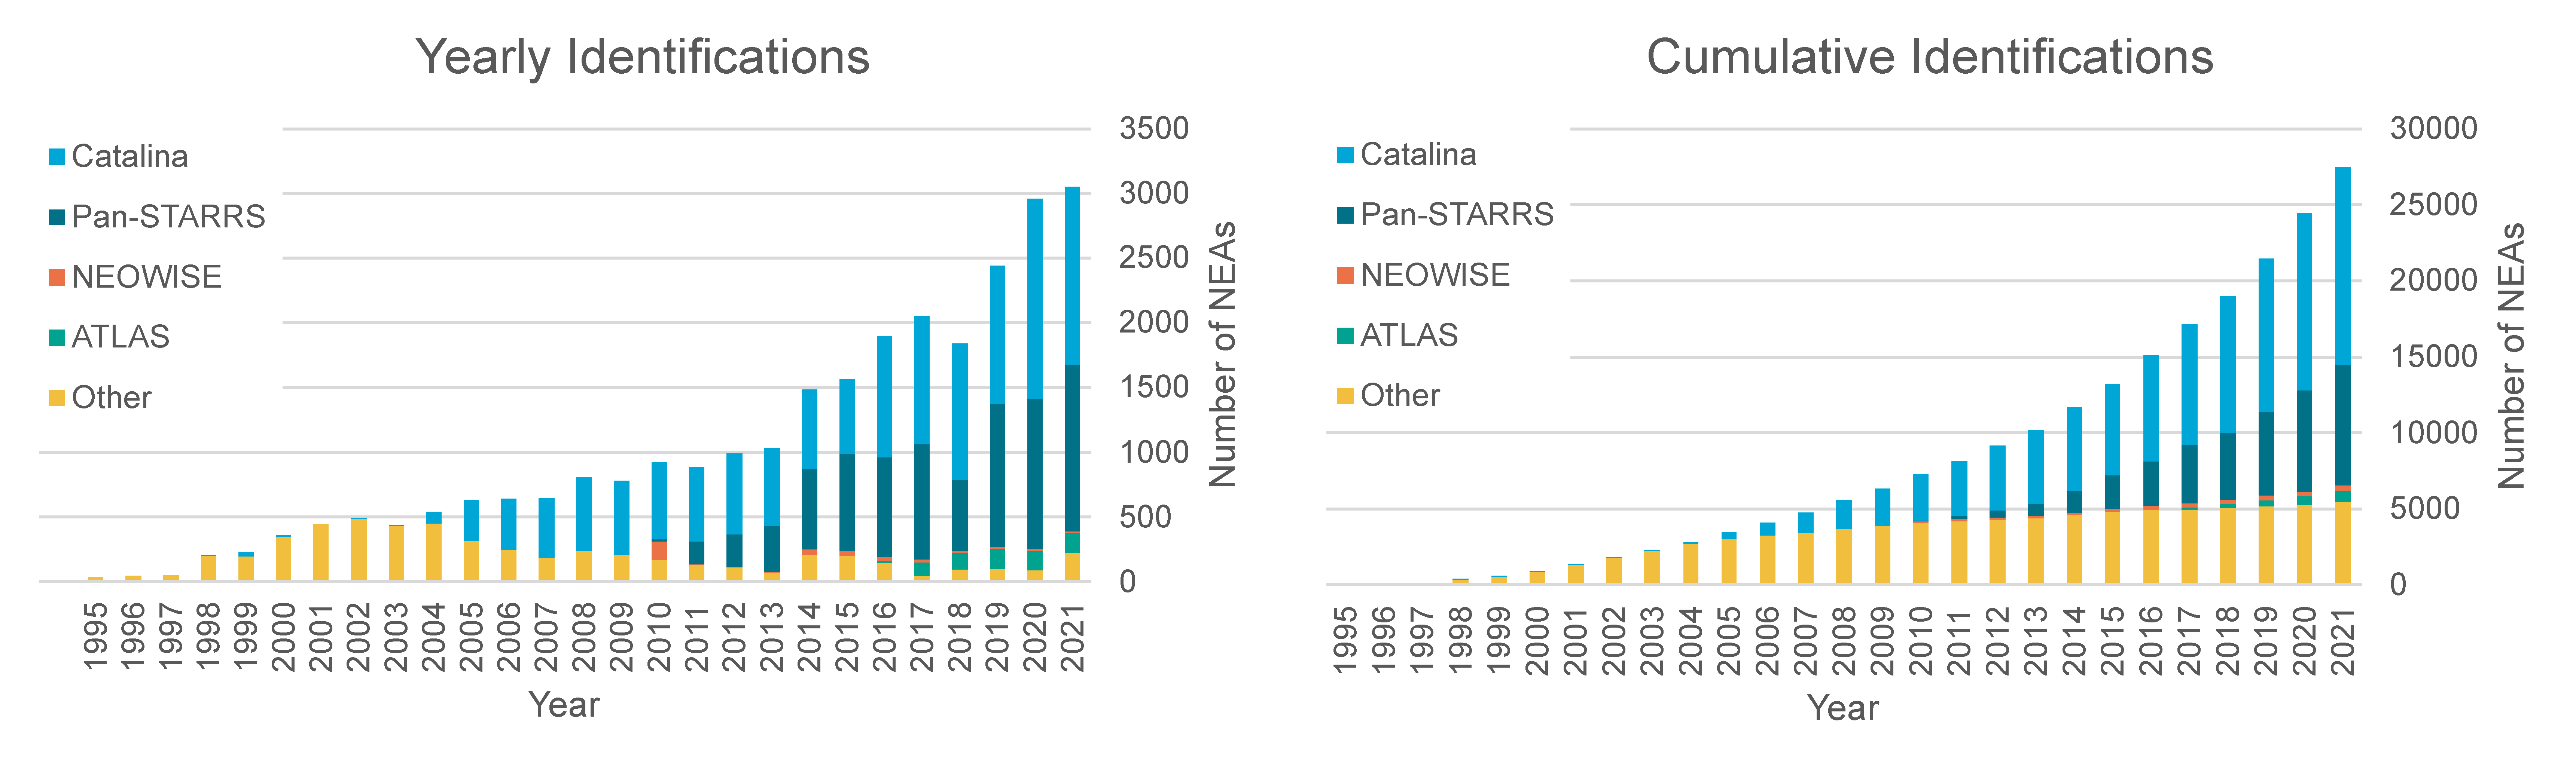
\includegraphics[width=1.0\textwidth]{img/identification_per_survey.pdf}
 \caption{Yearly and cumulative identifications made per NEA survey from 1995 up to and including 2021. Data obtained from \url{https://cneos.jpl.nasa.gov/stats}}
 \label{fig:identification_per_survey}
\end{figure}


\subsection{Earth-based Surveys}
With almost 13000 discoveries as of the end of 2021, the Catalina Sky Survey (CSS) is currently the most succesful NEA survey by volume of detections. Operated by the University of Arizona, the CSS operates a trio of telescopes in the Santa Catalina mountains: the primary telescope is a 1.5 meter wide field reflector telescope supported by a 1.0m follow-up telescope and a further 0.7m telescope, both catadioptric. The main telescope showcases the advantages of Earth-based surveys well, as it utilizes a 111 megapixel camera with a field of view of 5 square degrees. This allows it to image the sky at a very high frequency, down to a limiting magnitude of 21.5 (\cite{CatalinaSkySurvey}).\\

The second of the major NEA surveys is the Pan-STARRS project operated by the University of Hawaii. Operating two 1.8m catadioptric telescopes, equipped with 1.4 gigapixels camera sensors, it is capable of imaging down to a visual magnitude of 24. Currently, development is underway to expand Pan-STARRS to four telescopes, and allowing it to serve as a precursor for development of the software and data processing of the Large Synoptic Survey Telescope, which will be further discussed below (\cite{PANSTARRS}).\\

The last of the current large NEA surveys is the ATLAS (Asteroid Terrestrial-Impact Last Alert System) project. Contrary to the previously mentioned surveys, the goal of ATLAS is not to catalogue large quantities of NEA's, but to provide a last warning in case of incoming impactors. It is comprised of two 0.5m catadioptric telescopes, with plans to expand the system with three more sets of two telescopes. The survey is completely automated, and is tasked with providing impact warning for targets too small to observe until their last approach. The predicted warning times are between a day and a week (\cite{ATLAS}). Although this allows for alleviation of some of the damage, it is too short to take significant countermeasures such as an asteroid deflection mission or a large-scale evacuation. In addition, ATLAS suffers from the same problems as other Earth-based telescopes. For example, the 2013 Chelyabinsk meteor was not detected, as it approached Earth from the direction of the Sun, causing daylight to interfere with the observation.\\

Although not yet in operation, the expected impact of the Large Synoptic Survey Telescope (LSST) warrants mention. Currently being constructed in the mountains of Chile, the LSST will utilize a three-mirror reflector with a 8.4m aperture, in combination with a 3.2 gigapixel sensor, making it the largest digital camera ever produced. It is expected to enter operations fully in October 2023, with a limiting magnitude of around 24.5 (\cite{LSST}). Although the LSST is expected to complete the goal of cataloguing 90\% of the $D > 140 \mathrm{m}$ NEA population in approximately 12 years, it can be seen from its limiting magnitude that detecting the faintest of NEA's will not be a succesful endeavor for an Earth-based survey, even at extreme apertures and sensor sizes. Therefore, a short overview of some space-based surveys will now be provided.\\

\subsection{Space-based Surveys}
As shown above, meaningfully increasing the survey completeness for asteroids under the $D > 140 \mathrm{m}$ threshold is best carried out by means of a survey from space. To date, no dedicated NEA survey spacecraft has been launched, however, several missions have discovered a significant number of NEA's, most prominently among those the NEOWISE mission. Initially used for the WISE mission, imaging the entire sky in near-infrared, the spacecraft was put into hibernation after the coolant for its camera sensor ran out. In 2013, it was reawakened for the NEOWISE mission, where it would use its sensors in a non-cryogenic mode to survey for NEA's. Although the number of NEA's detected by NEOWISE is small compared to the dedicated Earth-based surveys, the new objects detected by it have been small and dark: targets which are hard to impossible to image using visual telescopes from Earth (\cite{NEOWISEResult}). NEOWISE thereby has shown the capability of both a space-based survey and a survey using near-infrared sensors, and its findings have contributed greatly to the capabilities for modelling the NEA population (e.g. \cite{GranvikPopulation}).\\

Building on the success of NEOWISE, a new spacecraft is currently being developed by NASA under the NEOCam project. Aiming for a launch in 2026, the NEOCam mission has a dedicated design for identification of NEA's. Situated at the Sun-Earth L1 point, the mission will observe the space around Earth for potentially hazardous asteroids. It is expected that NEOCam is also capable of completing the 90\% survey completeness of asteroids $D > 140 \mathrm{m}$, and will be capable of imaging some asteroids down to $D > 30 \mathrm{m}$, although the latter is not a primary design goal (\cite{NEOCam}).

\section{Possible Future Missions}
\label{sec:introductionproposals}
As an update to the new spaceguard objective, \cite{DefendingEarth} investigated the progress and goals of NEA cataloguing efforts. Their initial verdict was that current survey efforts are insufficient to meet the new goal, and new missions will be necessary. Several of these surveys have already been dicussed above. However, next to discussing NEA's with $D > 140 \mathrm{m}$, they also state that \textit{``... objects smaller than 140 meters in diameter are also capable of causing significant damage to Earth.''} and make the recommendation that \textit{``Because recent studies of meteor airbursts have suggested that near-earth objects as small as 30 to 50 meters in diameter could be highly destructive, surveys should attempt to detect as many 30- to 50-meter objects as possible.''}. \\

Leading among the current proposals is the work by NASA's Jet Propulsion Laboratory (\cite{2003NEOSDT}, \cite{2017NEOSDT}). The initial proposal centered around updating the limiting size of to-be-detected asteroids to lower limiting diameters. The authors investigate a multitude of possibilities for accomplishing the 90\% completeness at $D > 140 \mathrm{m}$ goal, as well as investigating the influence on smaller diameter asteroids. Their conclusion is in line with the aforementioned: the most promising option for cataloguing a multitude of NEA's is to perform a survey from deep space. Several options are considered, among which the best performing options are 0.5 meter aperture thermal infrared telescopes at Earth-Sun L1 or in Venus-trailing orbit. The authors note no significant gain in performance by increasing the aperture of the telescope further. It is also noted that no full optimization for the orbit or payload is performed. However, the proposal showcases the serious potential for deep-space NEA surveys. \\

\begin{figure}[htbp]
 \centering
 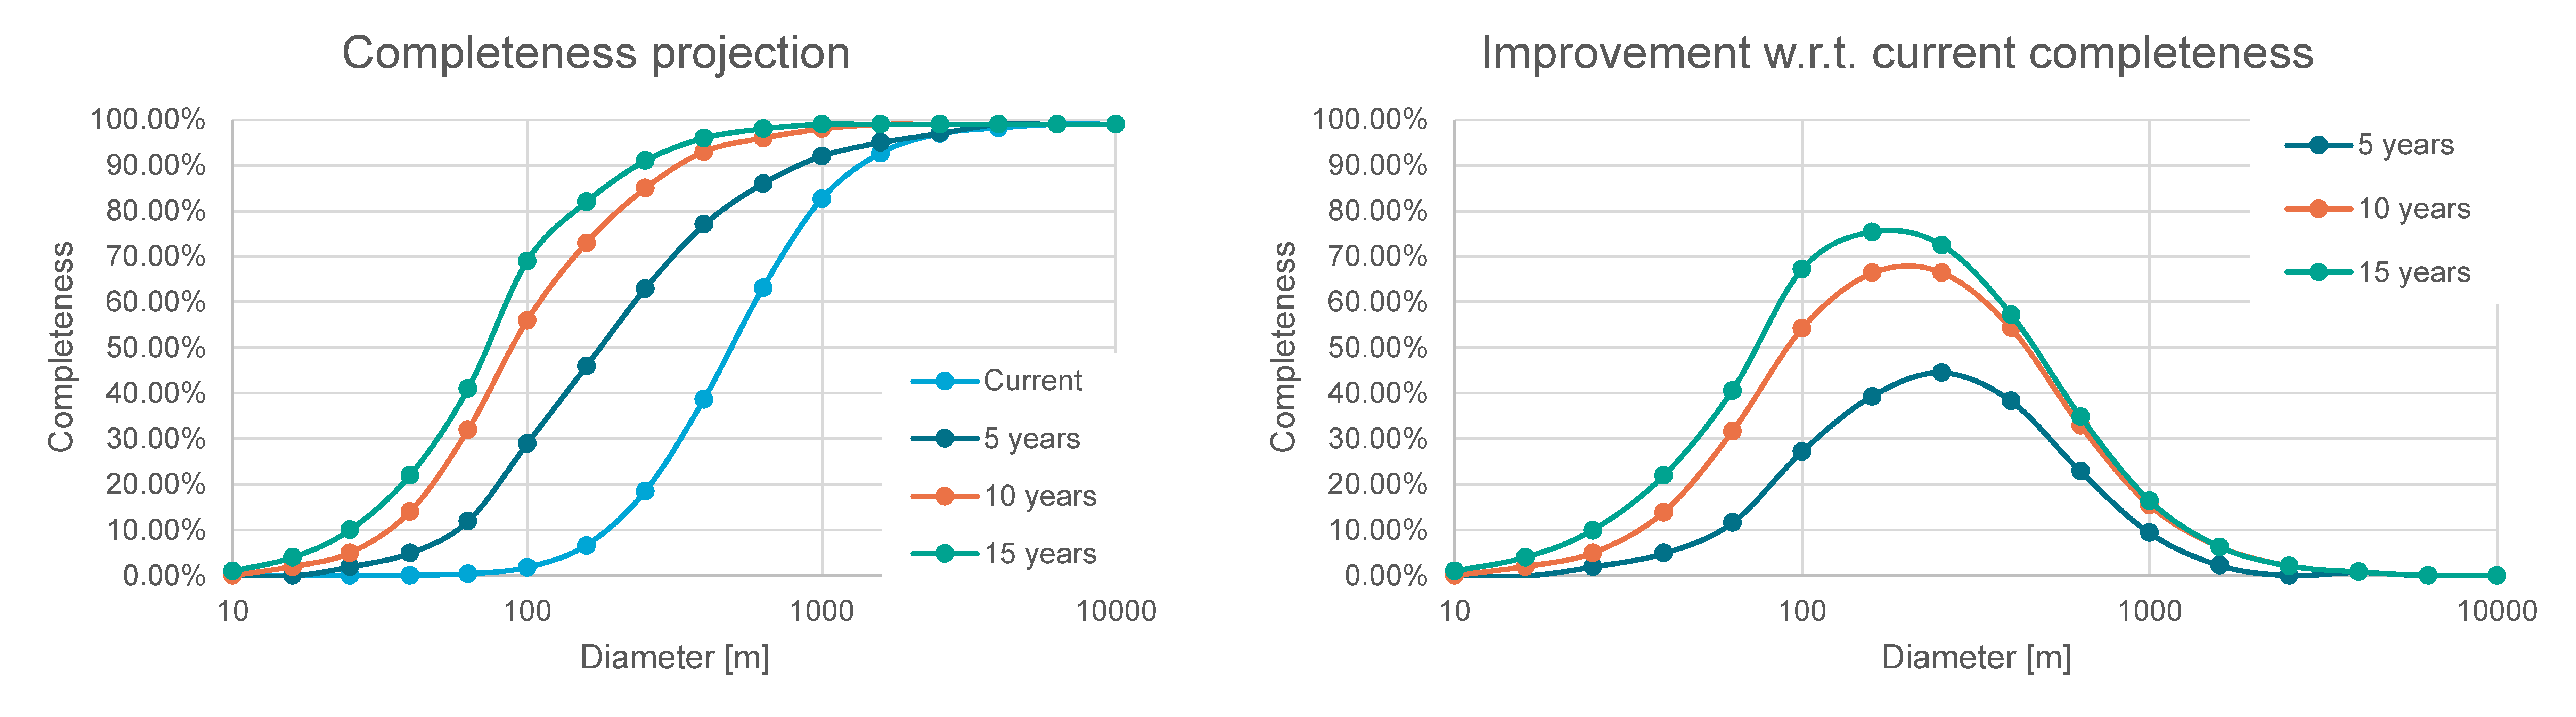
\includegraphics[width=1.0\textwidth]{img/completeness_projection.pdf}
 \caption{Projected improvement in survey completeness for a 5, 10 and 15 year survey from deep space. Data from \cite{2017NEOSDT}.}
 \label{fig:completeness_projection}
\end{figure}

\autoref{fig:completeness_projection} shows a projection for the improvement in survey completeness as a function of NEA diameter for a hypothetical deep space survey. A few thing are of note: Firstly, it is clear that such a survey can offer a sizeable improvement in cataloguing efforts, additionally leading to completion of the spaceguard goal in several years. However, several of the aforementioned missions currently under development also have this potential. What is more interesting is that, due to the thermal infrared telescope, cooled in deep space and largely free from interference by planets, is likely to detect a large number of small NEA's, which was hinted at by the success of the NEOWISE mission. But, the main bulk of the improvement is found in the $100 \mathrm{m} < D < 1000 \mathrm{m}$ range. Lastly, the diminishing returns of operating a mission for longer become clear: as the number of undetected NEA's which fall within the limiting magnitude of the detector decreases, the number of new NEA's detected in a given period of time decreases with it. \\

A second proposal among deep space surveys is the work of \cite{ThesisOlga}. The work investigates the problem of asteroid impact last warning from space. This addresses the weakness in systems such as ATLAS which was showcased by the Chelyabinsk impactor: If an asteroid approaches Earth from the Sun, it is not possible to detect it in advance from Earth, as the glare of the Sun will overpower the signal of the asteroid. They show that a system at the solar sail displaced Sun-Earth L1 point will provide good improvement to the effort of asteroid impact last warning strategies. However, as previously discussed, this would still leave insufficient time for e.g. a deflection mission (for the interested reader, \cite{DefendingEarth} gives a good overview of mitigation strategies). In addition, although the performance is vastly increased, performance in detecting asteroids coming from the direction of the Sun is still limited.\\

From the above, it is clear that current efforts are insufficient to reach the set goals for NEA cataloguing. In addition, although future surveys will reach this goal, they will only detect a small fraction of small NEA's, not cataloguing the largest population of near-Earth objects. In fact, even proposed surveys which avoid all interference from the atmosphere, the Earth and the Moon will not be capable of reaching this goal with a single spacecraft. Limitations are imposed by the location of the spacecraft, the required number of observations, and interference from Solar glare.



\section{The Small NEA Problem}
\label{sec:problemstatement}
The above leads to the following problem: Currently, humanity's knowledge of NEA populations is at a low level of completeness, especially for small diameter NEA's. Therefore, valuable scientific knowledge about the composition and evolution of the Solar system is unknown, and Earth is vulnerable to impacts which can be hazardous to human life and property. \\

It has been shown that current efforts are not adequate to reach the current goal of the spaceguard survey. Several missions have been proposed, and others are under development, which will cover this goal. However, a new more ambitious goal to identify smaller NEA's is still far out of reach. Even with a modern satellite positioned in deep space, only a limited survey completeness can be reached at limiting diameters $D < 100 \mathrm{m}$. This is caused by the limitations in position of this system, the required follow-up time and the number of detections required, and interference from the Sun.

\section{A Multi-Spacecraft Approach}
\label{sec:researchmultispacecraft}
To address this problem, we propose the option of a multi-spacecraft system. In recent years, spacecraft constellations have already shown a lot of potential in reaching complex mission goals. In the application of near-Earth asteroid surveys, more telescopes will firstly speed up the survey cadence, allowing the system to image the same area of sky at a faster rate. However, there are further synergystic advantages to such an approach. Three major benefits are noted in a multi-spacecraft system over a single telescope, which will be discussed in the following paragraphs.\\

Firstly, a multi-spacecraft system will mostly solve the problem of blind spots due to Solar glare and thermal limitations: Although a spacecraft in line with the Sun and an asteroid will not be able to detect the latter if it is located in the direction of the Sun, a different spacecraft located away from it might observe the Sun-asteroid arrangement from the side, allowing it to detect the target. In this way, a multi-spacecraft system is capable of minimizing the amount of blind spots in the search space. \autoref{fig:research_blind_spots} shows a visualisation of the reduction in blind areas when adding an additional spacecraft.\\

\begin{figure}[htbp]
 \centering
 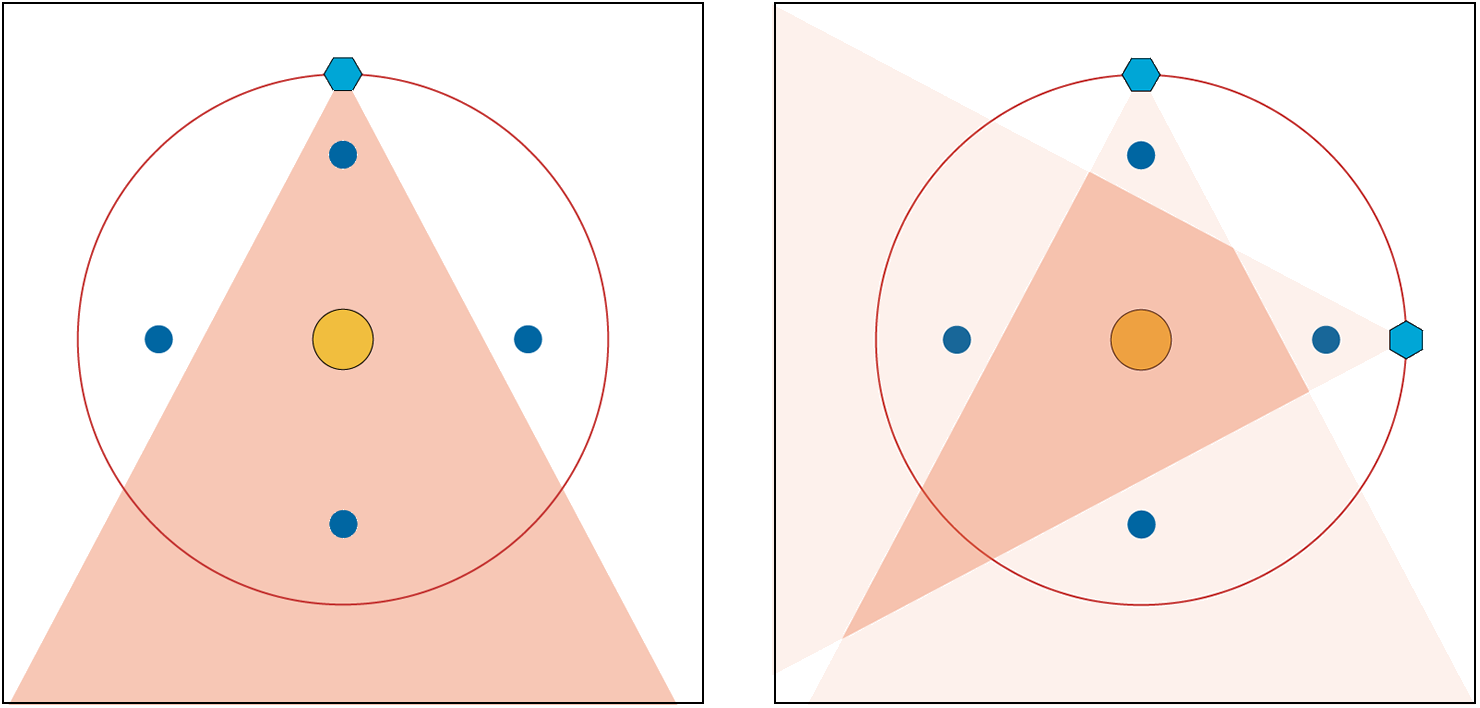
\includegraphics[width=0.8\textwidth]{img/research_blind_spots.png}
 \caption{Consider a spacecraft (represented by the cyan hexagon) attempting to observe several asteroids (blue circles). Because of Solar glare and thermal limits (red-shaded area), the spacecraft is unable to observe the top and bottom NEA. However, addition of a second spacecraft greatly reduces the ``blind area'': now the system can observe all four NEA's.}
 \label{fig:research_blind_spots}
\end{figure}


Secondly, using multiple spacecraft allows for easier identification and orbit determination of the NEA: Normally, a single telescope takes images in 2D of a target. As the asteroid will almost certainly be below the Rayleigh limit of the telescope, it is not possible to estimate how close the asteroid is from its estimated diameter and the projected size on the sensor: only the angular direction towards the target is known. Therefore, to obtain the orbit of the target requires solving Gauss' problem, which requires a minimum of three subsequent observations - six unknown parameters for the full orbit specification, two variables measured per observation. When observations from multiple spacecraft are used, it is possible to perform a process of triangulation, provided the spacecraft and the asteroid are not colinear. This allows for solving for the three-dimensional position of the asteroid. Thus, using only two observations in time reduces the orbit determination to Lambert's problem. This means the asteroid will only have to be within the area where telescopes can observe it for half the time as a single-spacecraft system. This is further shown in \autoref{fig:research_triangulation}, where addition of a second spacecraft allows for observing the asteroid before it moves out of the observable range.\\

\begin{figure}[htbp]
 \centering
 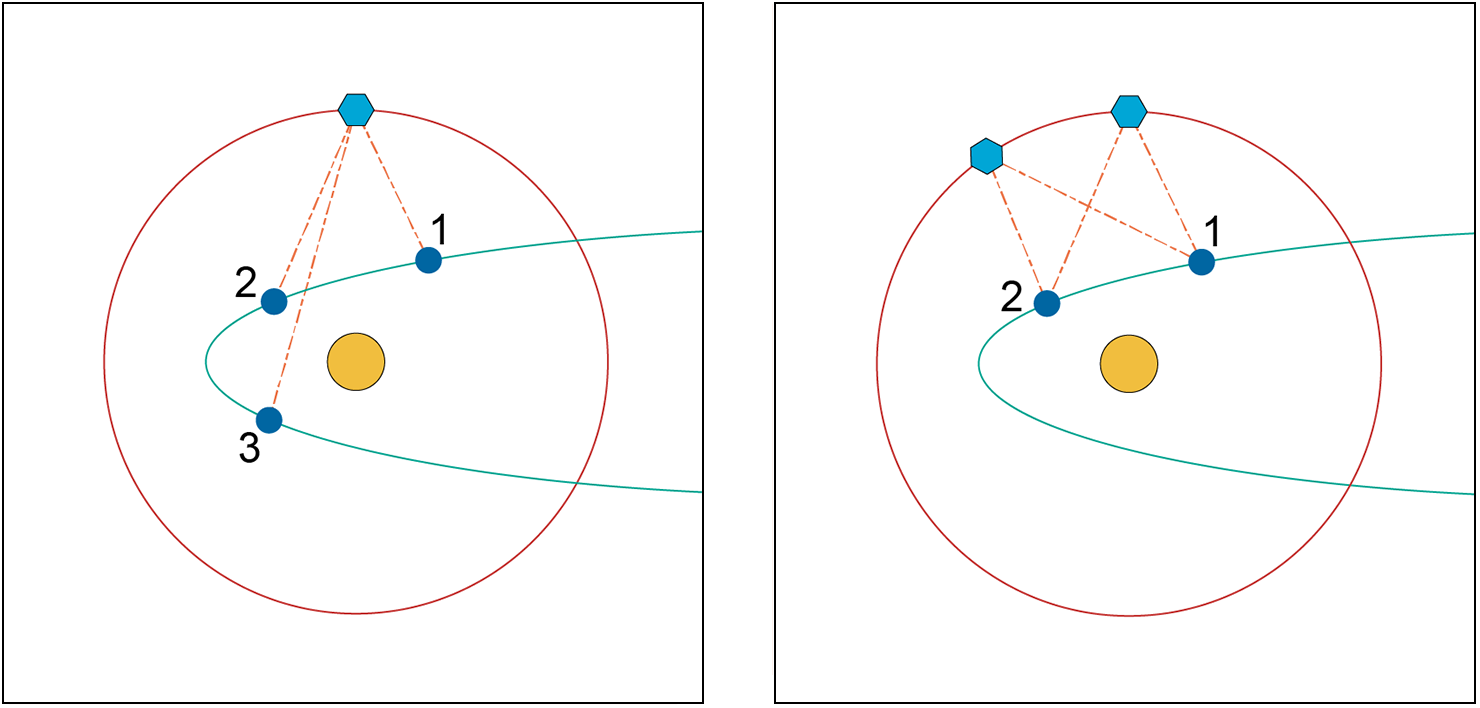
\includegraphics[width=0.8\textwidth]{img/research_triangulation.png}
 \caption{Normally, in order to perform orbit determination, the spacecraft (cyan hexagon) would have to image a target (blue cicle) three times. For targets that are hard to observe, such as a highly eccentric NEA which can only be detected close to perihelion, this leads to problems: the third detection will be hard to obtain, as the NEA moves behind the Sun into the blind area, or out of the detector's range altogether. Addition of a second spacecraft allows triangulation, thus halving the time required to identify the asteroid, performing the necessary measurements before the asteroid moves far away again.}
 \label{fig:research_triangulation}
\end{figure}


Lastly, a multi-spacecraft approach allows for more complex search strategies. The possibility for doing such search strategies when multiple telescopes are available is demonstrated by the Cataline Sky Survey. Using their follow-up telescope, a new target can be selected for follow-up imaging, quickly gathering the required observations to perform orbit determination and thereby identification. In space, such a strategy would of course be more complex, as the problem becomes influenced by the location of the spacecraft. However, such an implementation will be very helpful in detecting NEA's which are only visible for a short period of time, such as highly eccentric objects with long semi-major axes, which are only visible for a short window around their perihelion. This idea is demonstrated in \autoref{fig:research_search_strategy}.\\

\begin{figure}[htbp]
 \centering
 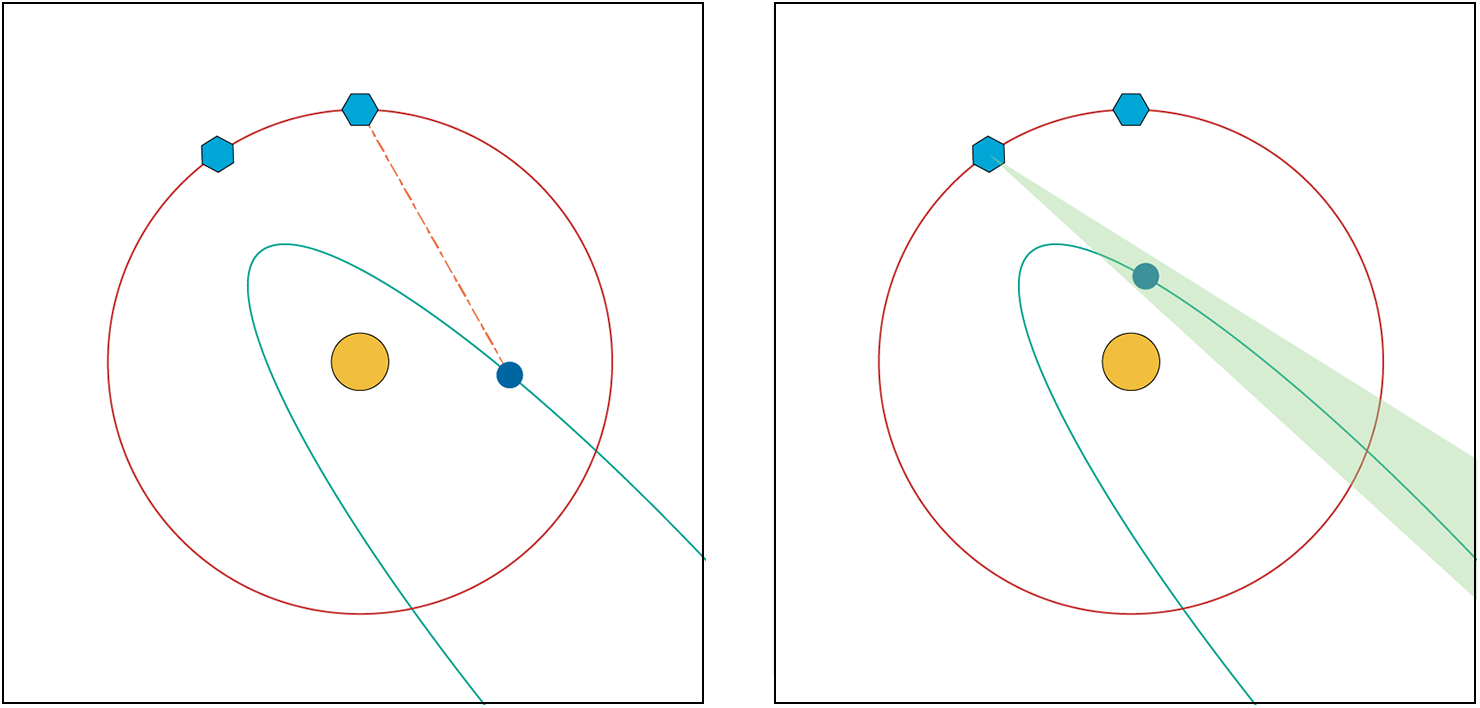
\includegraphics[width=0.8\textwidth]{img/research_search_strategy.png}
 \caption{In a more advanced system, some of the spacecraft could be dedicated to follow-up observations. As soon as one spacecraft detects a target, the second spacecraft is instructed to point in the direction of the new observation. In that way, even if a target is only observable for a short period, the spacecraft will have a much larger chance of pointing towards it.}
 \label{fig:research_search_strategy}
\end{figure}


However, before such strategies can be developed and implemented in a mission, it is first required to know the location and composition of such a multi-spacecraft system. To the author's best knowledge, the behavior of a multi-spacecraft survey has never been evaluated. In addition, to adequately assess the performance, it is vital to discover where the craft in such a system should be positioned, and how they should be equipped. The aim of this work are to provide insight into these points using simulation of such a survey.

\section{Research Questions and Expected Outcomes}
\label{sec:researchquestions}

To translate the aim into a concrete research topic, a main research question and a set of derived subquestions is composed. The main research question is:

\begin{center}\large\textbf{What is the optimal position and composition for a system of spacecraft with the purpose of identifying and cataloguing previously unidentified near-Earth asteroids?}\end{center}

A few terms deserve special attention: To begin, the terms \textit{position and composition} serve to indicate the scope of the research. As mentioned previously, no previous work has been published on multi-spacecraft NEA surveys. The current body of work on space-based surveys commonly uses general categories of orbits such as Venus-trailing orbits, or orbits at Lagrange points. In addition, either thermal infrared or a visual light telescope is used. In a multi-spacecraft system, the position should be treated in a more general sense: there is the added element of combining different positions synergistically, as explained in the previous section. Also, the composition with regards to payload is worthy of investigation: perhaps, a synergistic combination of slower but more sensitive infrared and faster but less sensitive visual light telescopes might be of merit. In addition to specifying what should be researched, these terms also limit the scope: other aspects, including - but not limited to - search strategy, communication between spacecraft, and image processing techniques will be left to further research. \\

The second factor of note is \textit{identifying and cataloguing}. The distinction between observation, detection, identification and cataloguing is worth the discourse before continuing. Essentially, these terms all represent successive steps in the survey. An \textit{observation} is when a target is within the telescope's field of view when an image is taken. Of course, this is not useful in and of itself. Therefore, a \textit{detection} can be established when the signal-to-noise ratio of the asteroid in the image is sufficiently high. At this point, it is clear that something is present in the telescope's field of view. When enough detections are established within a certain time frame, it becomes possible to determine the orbit of the target, and to see whether or not it is already known. At this point, an \textit{identification} can be performed from the subsequent observations. Then, with the orbit of the target known, the survey can proceed to \textit{cataloguing} the NEA by transmitting the relevant data back to Earth for analysis and storage. Thus, it is apparent that just observing or detecting an NEA is not useful in and of itself. For the information to be relevant, the system should be capable of contributing to the identification and cataloguing efforts. \\

The last term important to discuss before further explaining the research is \textit{unidentified} asteroids. As was discussed in \autoref{sec:introductionidentification}, humanity has already catalogued a sizeable portion of the NEA population. Naturally, it is not neccessary to identify these targets again. Therefore, the research effort should be concentrated on solving the identified problem of improving the knowledge of the small-diameter NEA population. \\

In support of the main research question, in conjunction with the aim of addressing the problem through a numerical simulation, several subquestions were drafted to assist in providing an answer. The first three subquestions are related to the design of the simulation; how to accurately produce and operate a model of NEA surveys. The next three questions are related to the parameters of such missions; where the spacecraft are located and how the system is composed. Lastly, a subquestion is included which will be essential for judging the results in the context of current and future endeavors, such as those listed in \autoref{sec:introductionidentification} and \autoref{sec:introductionproposals}. The subquestions are explained in brief below:
\begin{enumerate}
 \item \textbf{How can the population of NEA's be accurately modelled, and how can these models be adjusted for unidentified NEA's?}: The first subquestion is related to simulation. As mentioned above, the model needs to give an accurate estimate for how the system will perform in surveying unidentified NEA's. Therefore, first a model of this population is required. Although this may seem straightforward, it might pose some challenges: after all, only the identified portion of the NEA population is known, the unidentified portion is clearly not. Fortunately, literature sources are available to assist in this process.
 \item \textbf{How can surveys of NEA's by a system of spacecraft be accurately modelled?}: After modelling the asteroid population, the next consideration is how to model a survey of that population. Again, good sources in literature are available to assist in solving this question, although sufficient verification and validation will need to be performed.
 \item \textbf{How can the position and composition of the system be optimized?}: Already mentioned above, the possibilities for positioning and composing a multi-spacecraft system grow exponentially with the number of spacecraft in the system. Therefore, a good method of optimizing the system is required. It is expected that the simulation will be computationally expensive, and possibly noisy. Therefore, selection of a proper optimization method is crucial to ensure good results.
 \item \textbf{What is the effect of increasing the number of spacecraft on the process and performance of identifying and cataloguing NEA's?}: The first question related to the behavior of the system, and probably the most straightforward relation to consider when looking at the research question. Although it is apparent that an increase in the number of spacecraft will always increase the performance - or at worst, have it stay constant - the number of spacecraft is the most relevant free parameter to have results on, as it is a very important concept to explore and consider for future missions.
 \item \textbf{How is the performance of possible payload compositions affected by the number of spacecraft, and what is the resulting optimal payload composition?}: Secondly, the payload of the system. As explained in \autoref{sec:introductionproposals}, current research often uses either a visual or a thermal infrared telescope. However, when considering a multi-spacecraft system, combinations of these are possible. It will be good to see which of the systems benefits mostly from the increase in the number of spacecraft, and whether synergistic effects occur in hybrid systems composed of a mix of instrumentation. 
 \item \textbf{How do the number of spacecraft and payload interact with the orbital parameters of the system?}: The last of the free parameters is the positioning of the spacecraft. Next to studying the optimal position, it is also important to understand the behavior of the optimal orbital parameters as the number of spacecraft changes, as this is essential knowledge for a preliminary design effort.
 \item \textbf{How effective is a system of multiple spacecraft at identifying and cataloguing previously unidentified NEA's compoared to other current and future methods?}: A multi-spacecraft survey mission is a very costly endeavor, requiring several expensive spacecraft and the vehicles for launching these into outer space. Although this work will not go into detail on the economics of space missions, a realistic assessment to the merits of the idea should be made to consider whether it would be worth it to develop such a mission. 
\end{enumerate}

It is expected that through answering this research question, several outcomes will be obtained. The main goal is to provide outcomes which are useful in doing further research into, as well as designing, future NEA survey missions. The desired outcomes of this work are thus as follows:
\begin{enumerate}
 \item Understanding how increasing the number of spacecraft affects the performance of a NEA survey system. Of course, the performance will increase, however the main interest is in how much this performance increases, and thus whether such a solution is worth considering for future missions. It is expected that in addition to this, insight will be gained into any diminishing returns for higher numbers of spacecraft, and perhaps limits beyond which adding addition spacecraft provides no tangible benefit anymore.
 \item A conclusion on where to focus efforts with regards to payload. Currently, thermal infrared telescopes are considered the best choice for future NEA missions (e.g. \cite{2017NEOSDT}, \cite{ThesisOlga}). However, perhaps the benefits of a multi-spacecraft system are expressed stronger in a visual light system, or a hybrid system might provide a synergistic benefit.
 \item Insight into changes to the optimal orbital position for the spacecraft as a function of the number of spacecraft. It is expected that these quantities will undergo some change, and mapping this out allows for relating the results to the results of other studies on where to position NEA survey spacecraft.
 \item Reliable estimated for what performance to expect as a higher number of spacecraft is utilized in the system. In addition, this result is also interesting is reverse: seeing what kind of system would be necessary to obtain a desired result provides a basis for designing a mission out of such a requirement.
\end{enumerate}

Through fulfilling these goals and providing the expected outcomes, a useful base for further work on these kind of NEA surveys will thus be laid. In the next section, a short overview of the remainder of the report will be provided.

\section{Report Structure}
\label{sec:reportstructure}
The report is structured as follows: Firstly, in this chapter, the background of the problem and the multi-spacecraft concept was introduced. Additionally, a set of research questions and research aims was derived. In the next chapter, \autoref{ch:surveymodelling}, the theoretical background for modelling an asteroid survey from deep space will be given. This will cover the population model, the modelling of background and target signal, calculation of the signal-to-noise ratio, search strategy and cadence, and requirements for detection. Then, in \autoref{ch:experimental}, the methodology and implementation of the theory is provided. In particular, an overview will be given of the simulation's architecture, the implementation of all previously discussed components is explained, and the numerical optimization method is addressed. Lastly, the research process is discussed in more detail. \\

Following the modelling, in \autoref{ch:results}, the results of the simulation will be examined and discussed. In particular, findings will be done on the effect of the number of spacecraft in the system, the payload composition, and the orbital elements. In addition, an attempt will be made at explaining the findings through more fundamental principles, and the expected performance for future surveys will be predicted. To assure the reader of the accuracy of these conclusions, in \autoref{ch:vandv}, supplementary information on the verification and validation process is provided, along with inspection of the various assumptions made in the implementation. Lastly, in \autoref{ch:conclusion}, conclusions will be listed and the research questions answered. This will be supplemented by recommendations for further research. In addition to the main content, interested readers can find the full set of optimization results in \autoref{ch:appendix}.
